\section{贝叶斯回归}
\label{sec:regression-bayesian}

前面各模型给出一个点预测，并不说明这个预测有多大把握。贝叶斯回归为参数或函数设置先验，由数据得到后验分布，同时给出均值与不确定性。概率模型的基础见第\ref{sec:classic-overview-probability}节。

\subsection{贝叶斯线性回归}
\label{sec:regression-bayesian-linear}

\subsubsection{模型结构}
\label{sec:regression-bayesian-linear-structure}

设线性模型$\bm{y}=\widetilde{\bm{X}}\bm{\theta}+\bm{\varepsilon}$，$\bm{\varepsilon}\sim N(\bm{0},\sigma^2\bm{I})$，参数先验$\bm{\theta}\sim N(\bm{\theta}_0,\bm{\Sigma}_0)$，其中$\widetilde{\bm{X}}$是并入常数列后的$n\times(d+1)$设计。超参数$\sigma^2,\bm{\Sigma}_0$（如先验方差$\tau^2$）控制先验形状，与待推断的系数$\bm{\theta}$本身区分。要输出的不是一个最优向量，而是系数的后验分布，以及由此推出的新响应分布。高斯先验与高斯噪声共轭：先验与似然都是高斯，后验仍落在高斯族内，可解析写出；后验均值给出点估计，后验协方差给出各参数的不确定范围。

给定训练得到的系数后验$\bm{\theta}\mid\bm{y}\sim N(\widehat{\bm{\theta}}_N,\bm{\Sigma}_N)$（其推导见参数学习段；$\bm{\Sigma}_N$为$(d+1)\times(d+1)$的后验协方差），对新输入$\bm{x}_\star$先增广为$\widetilde{\bm{x}}_\star=(1,\bm{x}_\star^{\top})^{\top}$（与训练设计$\widetilde{\bm{X}}$同一列结构），预测规则为：预测均值$\widehat f(\bm{x}_\star)=\widetilde{\bm{x}}_\star^{\top}\widehat{\bm{\theta}}_N$；新响应$y_\star=\widetilde{\bm{x}}_\star^{\top}\bm{\theta}+\varepsilon_\star$同时含参数不确定性与新噪声，其方差为
\[
  \operatorname{Var}(y_\star\mid\bm{y})
  =\widetilde{\bm{x}}_\star^{\top}\bm{\Sigma}_N\widetilde{\bm{x}}_\star+\sigma^2.
\]
第一项来自后验协方差，第二项是独立观测噪声；二者相加才是对未来响应的预测方差。

由于后验是高斯的，$\bm{x}_\star^{\top}\bm{\theta}$与新噪声都为正态，未来响应条件分布为$N(\widehat f(\bm{x}_\star),\operatorname{Var}(y_\star\mid\bm{y}))$，按此正态分布即得预测区间；不能只报第一项。

\subsubsection{参数学习}
\label{sec:regression-bayesian-linear-learning}

\paragraph{系数后验}

后验密度正比于先验乘似然：$\log p(\bm{\theta}\mid\bm{y})\propto-\frac1{2\sigma^2}\lVert\bm{y}-\widetilde{\bm{X}}\bm{\theta}\rVert^2-\frac12(\bm{\theta}-\bm{\theta}_0)^{\top}\bm{\Sigma}_0^{-1}(\bm{\theta}-\bm{\theta}_0)$。把$\bm{\theta}$的二次项合并、一次项配方，恰好得到高斯的对数形式。零均值、各向同性先验$\bm{\theta}_0=\bm 0,\bm{\Sigma}_0=\tau^2\bm I$时，后验$\bm{\theta}\mid\bm{y}\sim N(\widehat{\bm{\theta}}_N,\bm{\Sigma}_N)$为
\begin{equation}
  \widehat{\bm{\theta}}_N
  =\left(\widetilde{\bm{X}}^{\top}\widetilde{\bm{X}}+\frac{\sigma^2}{\tau^2}\bm{I}\right)^{-1}
    \widetilde{\bm{X}}^{\top}\bm{y},
  \qquad
  \bm{\Sigma}_N
  =\sigma^2\left(\widetilde{\bm{X}}^{\top}\widetilde{\bm{X}}+\frac{\sigma^2}{\tau^2}\bm{I}\right)^{-1}.
  \label{eq:regression-bayesian-posterior}
\end{equation}
单截距例可复算精度相加。

设$\bm{y}=\mu\mathbf 1+\bm{\varepsilon}$，先验$\mu\sim N(0,\tau^2)$，观测精度$1/\sigma^2$、先验精度$1/\tau^2$在同一常数上合并，后验精度为$n/\sigma^2+1/\tau^2$，后验均值为$(n\bar y/\sigma^2)/(n/\sigma^2+1/\tau^2)$——样本多时由数据主导，样本小时回归先验原点。

\subsubsection{性质与先验选择}
\label{sec:regression-bayesian-linear-theory}

\paragraph{与二次正则的对应}

\begin{theorem}[高斯先验下的线性后验]
\label{thm:regression-bayesian-linear}
在高斯似然与高斯先验下，后验均值与协方差由式\eqref{eq:regression-bayesian-posterior}给出；MAP估计——最大后验，取后验分布的众数作为点估计——为
\begin{equation}
  \widehat{\bm{\theta}}_{\mathrm{MAP}}
  \in\arg\max_{\bm{\theta}}
  \left[-\frac{1}{2\sigma^2}\lVert\bm{y}-\tilde{\bm{X}}\bm{\theta}\rVert_2^2
    -\frac{1}{2\tau^2}\lVert\bm{\theta}\rVert_2^2\right],
  \label{eq:regression-map}
\end{equation}
其解与岭回归式\eqref{eq:regression-ridge-solution}在$\lambda=\sigma^2/(n\tau^2)$时一致。
\end{theorem}

\begin{proof}
对数后验等于对数似然加对数先验，略去常数后恰为平方数据项加二次惩罚；MAP取众数，而贝叶斯估计保留整个后验协方差。
\end{proof}

高斯后验的均值与MAP相同，一般先验中心和精度矩阵对应围绕该中心的二次正则。限定零均值、各向同性斜率先验，并把截距固定或采用平坦先验单独处理，就得到前文不惩罚截距的普通岭；任意正定先验对应任意二次惩罚，但不自动等于普通岭。图\ref{fig:regression-mle-map-geometry}比较MLE与MAP在参数平面上的位置：先验把估计从MLE向原点拉动。

\begin{figure}[htbp]
  \centering
  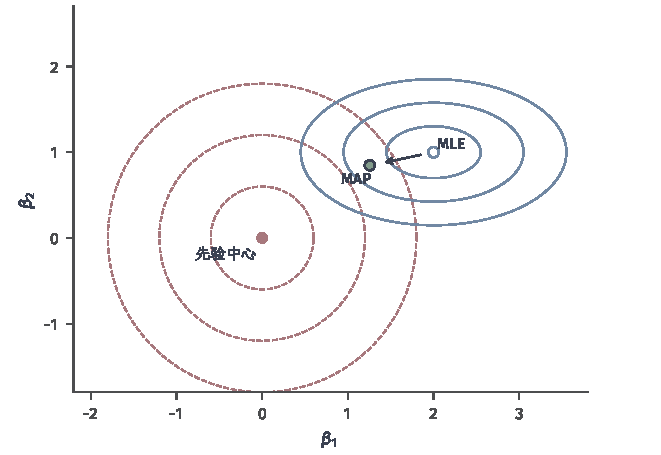
\includegraphics[width=105.412mm]{figures/04-classic-models/00-shared/matplotlib/regression-mle-map-geometry/figure.pdf}
  \caption{MLE与MAP的几何。等高线为似然椭圆，圆为各向同性先验约束；MLE取似然最高点，MAP取似然与先验联合最高处，位于MLE与原点之间。}
  \label{fig:regression-mle-map-geometry}
\end{figure}

\paragraph{不确定性的不同对象}

这里有三种容易混淆的方差：参数后验协方差$\bm{\Sigma}_N$描述$\bm{\theta}$在训练数据后的分布；重复抽样协方差描述频率学派在同一总体重采样下估计量的波动；新响应方差在上一段还叠加了观测噪声$\sigma^2$。区间的概率解释依赖所设先验、似然和超参数处理，不是任何固定真实机制下的频率保证；$\sigma^2,\tau^2$可由边缘证据（经验贝叶斯）估计。MAP只是后验众数，不等同于完整后验。

\subsection{高斯过程回归（GPR）}
\label{sec:regression-gpr}

贝叶斯线性回归的不确定性绑定在有限参数上；当关系是任意函数时，更自然的做法是直接把函数本身作为随机对象。\term{高斯过程回归}（Gaussian process regression, GPR）把先验放在函数上：任意有限输入处的函数值服从联合高斯，核规定两点函数值的协方差。Rasmussen与Williams在2006年给出高斯过程的系统论述\scite{rasmussen2006}。

\subsubsection{模型结构}
\label{sec:regression-gpr-structure}

有限高斯参数$f(\bm{x})=\phi(\bm{x})^{\top}\bm{w}$、$\bm{w}\sim N(\bm{0},\bm{\Sigma}_w)$诱导出协方差
\[
  \operatorname{Cov}(f(\bm{x}),f(\bm{x}'))=\phi(\bm{x})^{\top}\bm{\Sigma}_w\phi(\bm{x}');
\]
GPR直接规定任意有限输入上的函数值联合分布，不再显式写出参数。先验为
\[
  f(\cdot)\sim\mathcal{GP}(m_0(\cdot),C(\cdot,\cdot)),
\]
$m_0$为均值函数，$C$为合法协方差核。观测$y=f(\bm{x})+\varepsilon$，$\varepsilon\sim N(0,\sigma^2)$独立噪声。角色分三类：核矩阵$\bm{C}_{ij}=C(\bm{x}_i,\bm{x}_j)$由核函数与训练输入直接算出，是数据导出量；长度尺度$\ell$、信号幅度$s^2$、噪声方差$\sigma^2$等核超参数是待学参数；训练点的潜在函数值$\bm f$本身不显式待估，由先验与似然的后验给出。核$C$规定函数值随输入距离如何相关。

例如平方指数核$C(\bm{x},\bm{x}')=s^2\exp(-\lVert\bm{x}-\bm{x}'\rVert_2^2/(2\ell^2))$给出平滑、局部相关的函数：长度尺度$\ell$控制函数值在多远的距离上还显著相关，信号幅度$s^2$控制整体波动大小。观测分布$N(0,\sigma^2)$与函数先验是两件事，核只描述函数本身的协方差。

给定训练选定的核与噪声参数（核形式、长度尺度$\ell$、信号幅度$s^2$、噪声方差$\sigma^2$，由训练内超参数估计确定）、由训练输入直接算出的核矩阵$\bm{C}_{ij}=C(\bm{x}_i,\bm{x}_j)$、训练均值向量$\bm{m}_0=(m_0(\bm{x}_1),\ldots,m_0(\bm{x}_n))^{\top}$与训练响应$\bm{y}$（条件高斯配方见参数学习段），对新输入$\bm{x}_\star$的预测规则为
\begin{equation}
  \begin{aligned}
  \mu_\star
  &=m_0(\bm{x}_\star)+\bm{k}_\star^{\top}
    (\bm{C}+\sigma^2\bm{I})^{-1}
    (\bm{y}-\bm{m}_0),\\
  v_\star
  &=C_{\star\star}
    -\bm{k}_\star^{\top}
    (\bm{C}+\sigma^2\bm{I})^{-1}\bm{k}_\star,
  \end{aligned}
  \label{eq:regression-gp-posterior}
\end{equation}
其中$\bm{k}_\star=(C(\bm{x}_\star,\bm{x}_1),\ldots,C(\bm{x}_\star,\bm{x}_n))^{\top}$为新点到全部训练样本的核向量，$C_{\star\star}=C(\bm{x}_\star,\bm{x}_\star)$为新点自身的核方差。$\mu_\star$为函数后验均值（点预测），$v_\star$为函数方差；预测未来观测$y_\star=f_\star+\varepsilon_\star$时，$\varepsilon_\star\sim N(0,\sigma^2)$为独立新噪声，故未来响应均值仍为$\mu_\star$、方差为$v_\star+\sigma^2$。

图\ref{fig:regression-gp-posterior}展示式\eqref{eq:regression-gp-posterior}的两项输出：观测附近的函数值受到较强约束，观测间的较大空隙与远离观测的区域保留更多不确定性；曲线给出点预测，带状区域说明在当前先验和噪声设定下，哪些函数值仍与数据相容。

\begin{figure}[htbp]
  \centering
  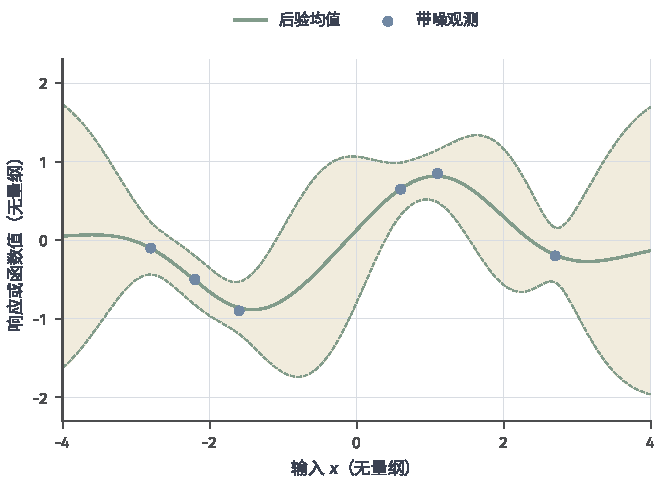
\includegraphics[width=105.412mm]{figures/04-classic-models/00-shared/matplotlib/regression-gp-posterior/figure.pdf}
  \caption{高斯过程后验。实线为后验均值，阴影为$\pm2\sqrt{v_\star}$函数方差带；观测附近带宽收窄，观测稀疏处带宽放宽。}
  \label{fig:regression-gp-posterior}
\end{figure}

\subsubsection{参数学习}
\label{sec:regression-gpr-learning}

\paragraph{潜在函数后验的条件高斯配方}

令$\bm{f}=(f(\bm{x}_1),\ldots,f(\bm{x}_n))^{\top}$，训练协方差矩阵$\bm{C}_{ij}=C(\bm{x}_i,\bm{x}_j)$。把训练响应$\bm y$与新点函数值$f_\star$放在同一个联合高斯里：均值分别为$\bm m_0$与$m_0(\bm x_\star)$，协方差分块为$\begin{bmatrix}\bm C+\sigma^2\bm I & \bm k_\star\\ \bm k_\star^{\top} & C_{\star\star}\end{bmatrix}$——左上是观测噪声与核叠加、右上是新点与训练记录的核。高斯分布条件化有现成规则：条件均值$=$原均值$+$交叉协方差$\times$观测协方差的逆$\times$（观测$-$观测均值），条件协方差$=$原协方差$-$交叉项$\times$逆$\times$自身，即“从先验方差里减去数据带来的信息”。按此规则条件化$\bm y$，即得模型结构段的式\eqref{eq:regression-gp-posterior}。

\paragraph{核与噪声超参数的学习}

给定核和噪声参数，后验已由式\eqref{eq:regression-gp-posterior}确定；仍需选择长度尺度$\ell$、信号方差$s^2$、噪声方差$\sigma^2$及可能的均值参数。直接追求训练拟合会把$\sigma^2$调到零、$\ell$调到极小，得到剧烈振荡的曲线。积分潜在函数得到边缘似然——把未知的潜在函数值$\bm f$积分掉后，只留下关于超参数的似然（零均值先验下）：
\begin{equation}
  \log p(\bm{y}\mid\bm{\theta})
  =-\frac12\bm{y}^{\top}\bm{C}_{\bm{\theta}}^{-1}\bm{y}
    -\frac12\log|\bm{C}_{\bm{\theta}}|
    -\frac n2\log 2\pi,
  \label{eq:regression-gp-evidence}
\end{equation}
$\bm{C}_{\bm{\theta}}=\bm{C}+\sigma^2\bm{I}$。第一项$\bm{y}^{\top}\bm{C}_{\bm{\theta}}^{-1}\bm{y}$衡量数据与核加噪声模型的匹配，拟合越好该项越小；第二项$\log|\bm{C}_{\bm{\theta}}|$是归一化项，协方差过大（核过度灵活）时该项也大，从而惩罚无依据的复杂度。从矩阵微分求超参数梯度。记$\bm{a}=\bm{C}_{\bm{\theta}}^{-1}\bm{y}$，对式\eqref{eq:regression-gp-evidence}关于$\theta_j$求导得
\[
  \frac{\partial\log p}{\partial\theta_j}
  =\frac12\bm{a}^{\top}
    \frac{\partial\bm{C}_{\bm{\theta}}}{\partial\theta_j}\bm{a}
   -\frac12\operatorname{tr}\left(
     \bm{C}_{\bm{\theta}}^{-1}
     \frac{\partial\bm{C}_{\bm{\theta}}}{\partial\theta_j}
   \right),
\]
沿增大边缘似然的方向迭代。正参数（长度尺度、方差）在优化时取对数坐标，初值由训练集量级粗定，最终在留出数据上检查。

\paragraph{矩阵计算与数值实现}

使用Cholesky分解计算拟合与新点预测：先对正定的$\bm{C}_{\bm{\theta}}=\bm{C}+\sigma^2\bm{I}$作Cholesky分解——把正定矩阵写成下三角与其转置之积——再回代求解线性系统，避免直接求逆；单点均值与方差各自的代价分别为$O(n^2)$与$O(n^3)$量级，存储与求逆随$n$增长。

\subsubsection{理论分析}
\label{sec:regression-gpr-theory}

\paragraph{有限基模型与GP}

有限高斯参数$f(\bm{x})=\phi(\bm{x})^{\top}\bm{w}$、$\bm{w}\sim N(\bm{0},\bm{\Sigma}_w)$诱导出协方差
\[
  \operatorname{Cov}(f(\bm{x}),f(\bm{x}'))=\phi(\bm{x})^{\top}\bm{\Sigma}_w\phi(\bm{x}'),
\]
即有限基线性模型在函数值上诱导出一个核；反过来，任取该形式的核，对应的GP后验与该有限基模型的参数后验一一对应。GPR不显式限制基，核直接规定函数协方差。核秩不足或设计退化时，有效自由度少于形式维度，需按有效秩处理。

\paragraph{后验方差与模型条件}

$v_\star=C(\bm{x}_\star,\bm{x}_\star)-\bm{k}_\star^{\top}(\bm{C}+\sigma^2\bm{I})^{-1}\bm{k}_\star$是先验核方差减去数据提供的信息，因核矩阵半正定而恒非负。观测密集且核相关强的方向，$v_\star$小；远离观测或核相关弱的区域，$v_\star$保留先验大小。后验方差只反映函数估计的不确定性，不度量未来噪声；模型内概率不能直接变成任意固定真实机制下的频率覆盖保证。核的平滑假设、观测分布失配与超参数点估计忽略的不确定性，都会使理论计算精确与真实任务预测正确之间存在差距。

\paragraph{与核岭点预测的对应}

同一个零均值后验均值还可由核岭回归求得。在第\ref{sec:regression-krr}节的核空间中使用平方损失而非SVR容忍带，目标为
\[
  \min_f\frac{1}{2n}\sum_i(y_i-f(\bm{x}_i))^2+\frac{\lambda}{2}\lVert f\rVert_{\mathcal H_k}^2,
\]
其解为$f(\bm{x}_\star)=\bm{k}_\star^{\top}(\bm{K}+n\lambda\bm{I})^{-1}\bm{y}$。在两者均使用已知零均值、相同核且GP噪声方差满足$\sigma^2=n\lambda$时，比较$\bm{k}_\star^{\top}(\bm{K}+\sigma^2\bm{I})^{-1}\bm{y}$与前面固定零截距的核岭解，说明相同点预测的条件与参数换算；这只是点预测的对应：核岭没有因此获得GP后验协方差，GP样本路径也不能直接等同于RKHS中的确定函数；非零均值需先拟合$\bm{y}-m_0$再加回。

\subsubsection{支持非高斯响应：改变似然与近似后验}
\label{sec:regression-gp-nongaussian}

\paragraph{改变似然后的计算困难}

设先验$\bm f\sim N(\bm 0,\bm C)$、观测$\bm y$因子化似然$p(\bm y\mid\bm f)=\prod_i p(y_i\mid f_i)$。响应非高斯（Poisson计数、二分类）时，似然不再与高斯先验共轭：以Poisson为例，$\log p(y_i\mid f_i)=y_i f_i-e^{f_i}-\log(y_i!)$中$e^{f_i}$对$f_i$不是二次的，后验
\[
  p(\bm f\mid\bm y)\propto p(\bm y\mid\bm f)\,N(\bm f\mid\bm 0,\bm C)
  =\exp\!\left(\sum_i y_i f_i-e^{f_i}-\tfrac12\bm f^{\top}\bm C^{-1}\bm f\right)
\]
无法配成高斯，后验均值、方差与新点预测都没有闭式。下面两条路线都把后验替换成一条可处理的高斯曲线，差别在替换的位置：Laplace只在众数附近展开，变分按整条分布的KL距离衡量。

\paragraph{Laplace近似：众数处的局部高斯}

第一步写出待最大化的目标。略去常数，取对数后验
\[
  \Psi(\bm f)=\log p(\bm y\mid\bm f)-\tfrac12\bm f^{\top}\bm C^{-1}\bm f,
\]
最大化$\Psi$就是求后验众数$\widehat{\bm f}$。

第二步求一阶条件。梯度为
\[
  \nabla\Psi(\bm f)=\nabla\log p(\bm y\mid\bm f)-\bm C^{-1}\bm f,
\]
令其为零：众数满足$\widehat{\bm f}=\bm C\,\nabla\log p(\bm y\mid\widehat{\bm f})$——依据是$\bm C^{-1}\bm f=\nabla\log p(\bm y\mid\bm f)$两边左乘$\bm C$。

第三步写出二阶导。因子化似然下定义对角矩阵$\bm W=-\nabla\nabla^{\top}\log p(\bm y\mid\bm f)$（对角元为$-{\partial^2\log p(y_i\mid f_i)}/{\partial f_i^2}$），则
\[
  \nabla^2\Psi(\bm f)=-\bm W-\bm C^{-1}.
\]
两个具体形式：Poisson有$W_{ii}=e^{f_i}$；logistic伯努利有$W_{ii}=\pi_i(1-\pi_i)$，其中$\pi_i=\sigma(f_i)$。

第四步用牛顿法迭代到众数。令$\bm g=\nabla\log p(\bm y\mid\bm f)-\bm C^{-1}\bm f$、$\bm H=\bm W+\bm C^{-1}$为负的二阶导，牛顿更新$\bm f_{\text{new}}=\bm f+\bm H^{-1}\bm g$，代入$\bm g$并整理（依据：$\bm f=\bm H^{-1}\bm H\bm f$）得
\[
  \bm f_{\text{new}}=(\bm C^{-1}+\bm W)^{-1}\big(\bm W\bm f+\nabla\log p(\bm y\mid\bm f)\big);
\]
每次迭代在当前$\bm f$处重算$\bm W$与梯度，直至收敛到$\widehat{\bm f}$。

第五步把后验换成众数处的二阶展开。依据泰勒公式：$\Psi(\bm f)\approx\Psi(\widehat{\bm f})-\tfrac12(\bm f-\widehat{\bm f})^{\top}\bm H(\bm f-\widehat{\bm f})$，即近似后验
\[
  q(\bm f)=N\big(\widehat{\bm f},(\bm C^{-1}+\bm W)^{-1}\big),
\]
其中$\bm W$在$\widehat{\bm f}$处取值；$\bm H$正定才能定义这条高斯，秩不足时只能覆盖部分方向。

数值上不直接求$(\bm C^{-1}+\bm W)^{-1}$：令$\bm B=\bm I+\bm W^{1/2}\bm C\bm W^{1/2}$（$\bm W$对角，平方根为对角阵），由Woodbury恒等式
\[
  (\bm C^{-1}+\bm W)^{-1}=\bm C-\bm C\bm W^{1/2}\bm B^{-1}\bm W^{1/2}\bm C.
\]
$\bm B$与$\bm C$同为$n\times n$，并非更小；它的好处是特征值全部不小于$1$、条件数良好，而且既不要求求$\bm C^{-1}$，也不要求求$\bm W^{-1}$（$\bm W$含零元时$\bm W^{-1}$根本不存在）。实际计算对$\bm B$作Cholesky分解$\bm B=\bm L\bm L^{\top}$，$\log\det\bm B=2\sum_i\log L_{ii}$。同时$\log\det\bm H=\log\det\bm C^{-1}+\log\det\bm B$。近似对数边缘似然为
\[
  \log q(\bm y)=-\tfrac12\widehat{\bm f}^{\top}\bm C^{-1}\widehat{\bm f}
  +\log p(\bm y\mid\widehat{\bm f})-\tfrac12\log\det\bm B,
\]
由它对核参数（长度尺度、信号幅度）求导，把超参数学习与近似后验放在同一目标里。

第六步给出新点预测。依据联合高斯条件化与Woodbury恒等式，潜在函数在新输入$\bm x_\star$处的近似后验为
\[
  \mu_\star=\bm k_\star^{\top}\nabla\log p(\bm y\mid\widehat{\bm f}),
  \qquad
  v_\star=C_{\star\star}-\bm k_\star^{\top}(\bm C+\bm W^{-1})^{-1}\bm k_\star,
\]
$\bm k_\star$为新点到训练样本的核向量、$C_{\star\star}=C(\bm x_\star,\bm x_\star)$。上式中$(\bm C+\bm W^{-1})^{-1}$同样由Woodbury恒等式化为不含$\bm W^{-1}$的稳定形式
\[
  v_\star=C_{\star\star}-\bm k_\star^{\top}\bm W^{1/2}\bm B^{-1}\bm W^{1/2}\bm k_\star,
\]
$\bm W$含零元（某些观测的曲率为零）时用此式计算。注意这只是潜在函数的近似后验：预测响应时还要对似然积分。以Poisson为例，$E[e^{f_\star}]=e^{\mu_\star+v_\star/2}$（高斯变量的指数的均值），均值预测为该值，不是$\mu_\star$本身。

\paragraph{变分近似：整体拟合的高斯$q$}

Laplace只在众数附近展开；变分近似则直接限制候选分布族为$q(\bm f)=N(\bm m,\bm S)$，并最小化它与真实后验的KL散度。由恒等式
\[
  \log p(\bm y)-\mathrm{ELBO}=\mathrm{KL}(q(\bm f)\Vert p(\bm f\mid\bm y)),
\]
\[
  \mathrm{ELBO}=\mathbb E_q[\log p(\bm y\mid\bm f)]-\mathrm{KL}(q(\bm f)\Vert p(\bm f));
\]
左边$\log p(\bm y)$与$q$无关，故最大化ELBO恰好等价于最小化$\mathrm{KL}(q\Vert p(\bm f\mid\bm y))$，即高斯族内最接近真实后验。先验$p(\bm f)=N(\bm 0,\bm C)$与$q$都是高斯，两项高斯的KL有闭式
\[
  \mathrm{KL}(q\Vert p)=\tfrac12\big(\operatorname{tr}(\bm S\bm C^{-1})+\bm m^{\top}\bm C^{-1}\bm m-n-\log\det\bm S+\log\det\bm C\big).
\]

因子化似然下，期望项拆成互不耦合的一维积分：$\mathbb E_q[\log p(y_i\mid f_i)]$只需$f_i\sim N(m_i,S_{ii})$。Poisson有闭式$y_i m_i-\exp(m_i+S_{ii}/2)$（依据：高斯变量的一阶矩与指数矩）；伯努利没有闭式，用Gauss--Hermite求积对该一维高斯数值积分。对$\bm S$求ELBO的稳定点：由矩阵微商$\partial\mathrm{ELBO}/\partial\bm S=\tfrac12\mathbb E_q[\nabla^2\log p(\bm y\mid\bm f)]-\tfrac12\bm C^{-1}+\tfrac12\bm S^{-1}=\bm 0$，得
\[
  \bm S=(\bm C^{-1}+\bm\Lambda)^{-1},
\]
$\bm\Lambda$为对角阵，$\Lambda_{ii}=-\mathbb E_q[\partial^2\log p(y_i\mid f_i)/\partial f_i^2]\ge0$（似然的二阶导为负，故$\bm\Lambda$非负）；$\bm m$沿$\partial\mathrm{ELBO}/\partial\bm m=\mathbb E_q[\nabla\log p(\bm y\mid\bm f)]-\bm C^{-1}\bm m$迭代。$\bm m,\bm S,\bm\Lambda$互相依赖，固定其他量轮流更新至收敛。

与Laplace的区别：Laplace只用后验众数一点的局部曲率，近似后验只保证在众数附近贴合；变分按整条$q$计算KL距离，似然期望对整个$q$取平均，代价是每步期望要对一维高斯求积分。


\subsubsection{支持更多观测：诱导变量近似}
\label{sec:regression-gp-computation}

\paragraph{诱导变量与近似族}

精确GPR的协方差求逆为$O(n^3)$，完整核矩阵的时间与存储压力推动近似。诱导变量方法选$m\ll n$个诱导位置$\bar{\bm{x}}_j$，引入少数位置上的函数值而不是丢掉其他观测；其动机是Nyström近似：训练点间的完整核矩阵可由诱导点重构为$\bm C\approx\bm C_{nm}\bm C_{mm}^{-1}\bm C_{mn}$（$\bm C_{mm}$为诱导点两两核、$\bm C_{nm}$为训练—诱导跨块核），于是完整求逆被$m\times m$求逆替代。诱导值$\bm{u}=(f(\bar{\bm{x}}_1),\ldots,f(\bar{\bm{x}}_m))^{\top}$，定义训练潜在函数值$\bm{f}$、诱导值$\bm{u}$及近似族$q(\bm{f},\bm{u})=p(\bm{f}\mid\bm{u})q(\bm{u})$，保留先验条件分布$p(\bm{f}\mid\bm{u})$，全部观测仍进入学习，$q(\bm{u})$为高斯，其均值与协方差为待学参数\scite{titsias2009}。

\paragraph{变分下界与训练}

由联合后验KL非负，$\log p(\bm{y})$的ELBO为
\[
  \mathrm{ELBO}=\mathbb E_{q(\bm f,\bm u)}[\log p(\bm y\mid\bm f)]
  -\mathrm{KL}\big(q(\bm f,\bm u)\Vert p(\bm f,\bm u)\big),
\]
间隙为$\mathrm{KL}(q(\bm f,\bm u)\Vert p(\bm f,\bm u\mid\bm y))$。对第二个KL按链式规则分解：
\[
  \mathrm{KL}\big(q(\bm f,\bm u)\Vert p(\bm f,\bm u)\big)
  =\mathrm{KL}\big(q(\bm u)\Vert p(\bm u)\big)
  +\mathbb E_{q(\bm u)}\big[\mathrm{KL}\big(q(\bm f\mid\bm u)\Vert p(\bm f\mid\bm u)\big)\big].
\]
近似族令$q(\bm f\mid\bm u)=p(\bm f\mid\bm u)$（保留先验条件分布），第二项恒为零——这就是"共同条件分布抵消"；观测似然只依赖$\bm f$，期望化为$\mathbb E_{q(\bm u)}\mathbb E_{p(\bm f\mid\bm u)}[\log p(\bm y\mid\bm f)]$。于是目标只剩
\[
  \mathbb E_q[\log p(\bm y\mid\bm f)]-\mathrm{KL}(q(\bm u)\Vert p(\bm u)).
\]
固定核时学$q(\bm u)$参数，诱导位置与核由训练内验证选择；新输入经$q(\bm u)$传播得到近似均值与方差，计算代价降为$O(nm^2)$，点预测与方差近似需分别验证。
